\section{Motion \& Temporal Dynamics}
\begin{frame}{}
    \LARGE Video Learning \& Generation: \textbf{Motion \& Temporal Dynamics}
\end{frame}

\begin{frame}{Recognising Actions from Motion}
    \begin{itemize}
        \item Motion as a primary cue for recognising actions in videos.
        \item Importance of separating the analysis of appearance and motion.
        \item Motion patterns often provide more discriminative information than static appearance.
    \end{itemize}
\end{frame}

\subsection{Optical Flow}
\begin{frame}{Measuring Motion: Optical Flow}
    \begin{itemize}
        \item Computes a dense motion field between consecutive frames.
        \item Popular algorithms:
        \begin{itemize}
            \item Farneback
            \item TV-L1
        \end{itemize}
        \item Optical flow is commonly used as input to Two-Stream Networks for action recognition.
    \end{itemize}
\end{frame}

\begin{frame}[allowframebreaks]{Optical Flow: Key Concepts}
    \begin{itemize}
        \item \textbf{Dense Motion Field}: Represents motion vectors for every pixel between two frames.
        \item \textbf{Temporal Coherence}: Assumes that motion is smooth and continuous over time.
        \item \textbf{Applications}: Used in action recognition, video segmentation, and object tracking.
    \end{itemize}
\framebreak
    \begin{figure}
        \centering
        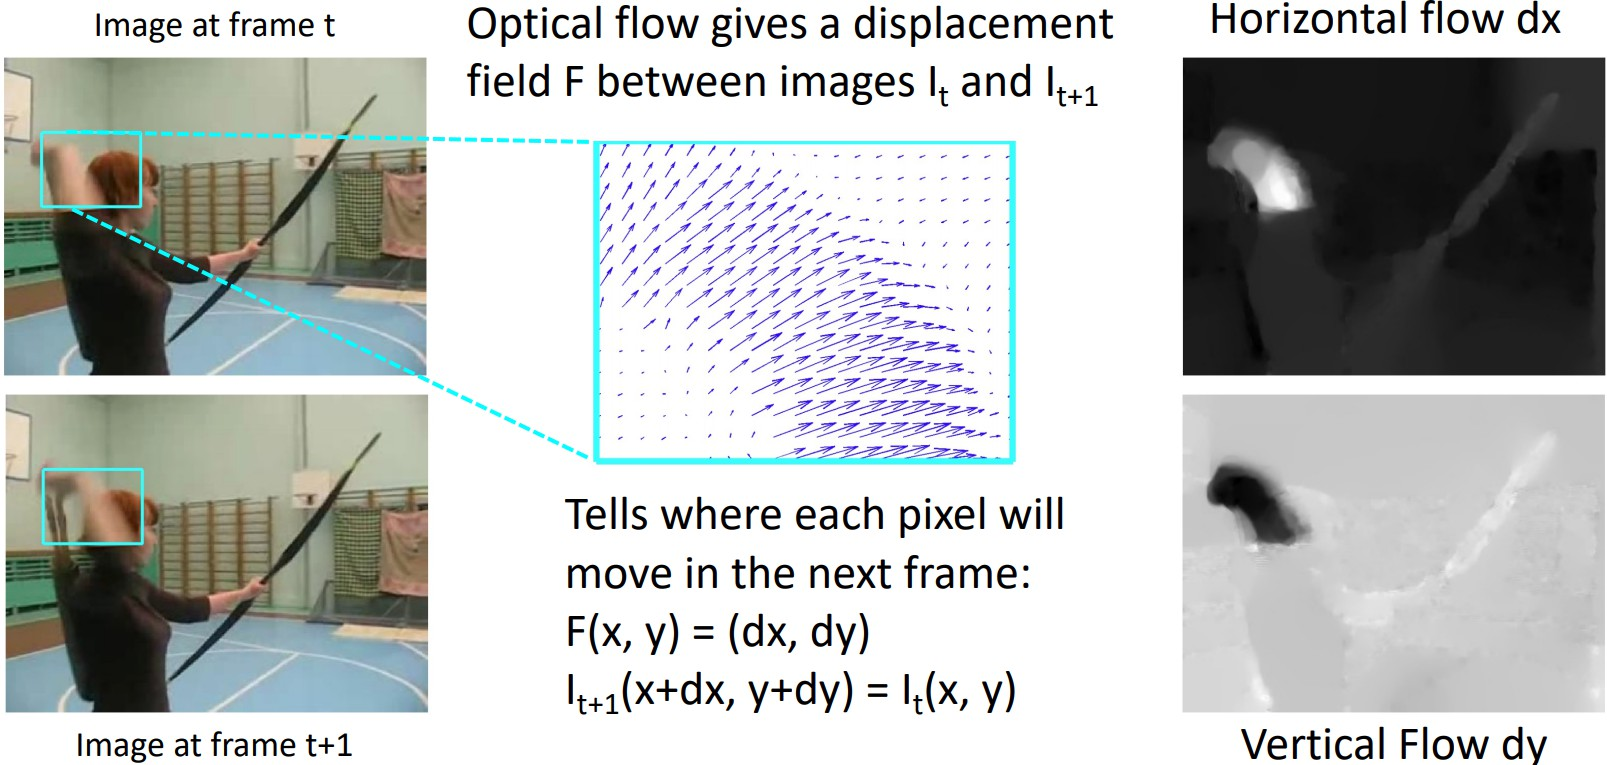
\includegraphics[width=1\textwidth,height=0.9\textheight,keepaspectratio]{images/video/slide_22_1_img.jpg}
    \end{figure}
\end{frame}
\subsection{Two-Stream Networks}
\begin{frame}{Separating Motion and Appearance}
    \begin{itemize}
        \item \textbf{Two-Stream Network:} Processes both RGB (appearance) and optical flow (motion) streams.
        \item Streams can be fused at various depths:
        \begin{itemize}
            \item \textit{Early fusion:} Combine features at initial layers.
            \item \textit{Late fusion:} Combine predictions or high-level features.
        \end{itemize}
        \item Improves robustness to background and enhances motion understanding.
    \end{itemize}
\end{frame}

\begin{frame}[allowframebreaks]{Two-Stream Network Architecture}
    \begin{figure}
        \centering
        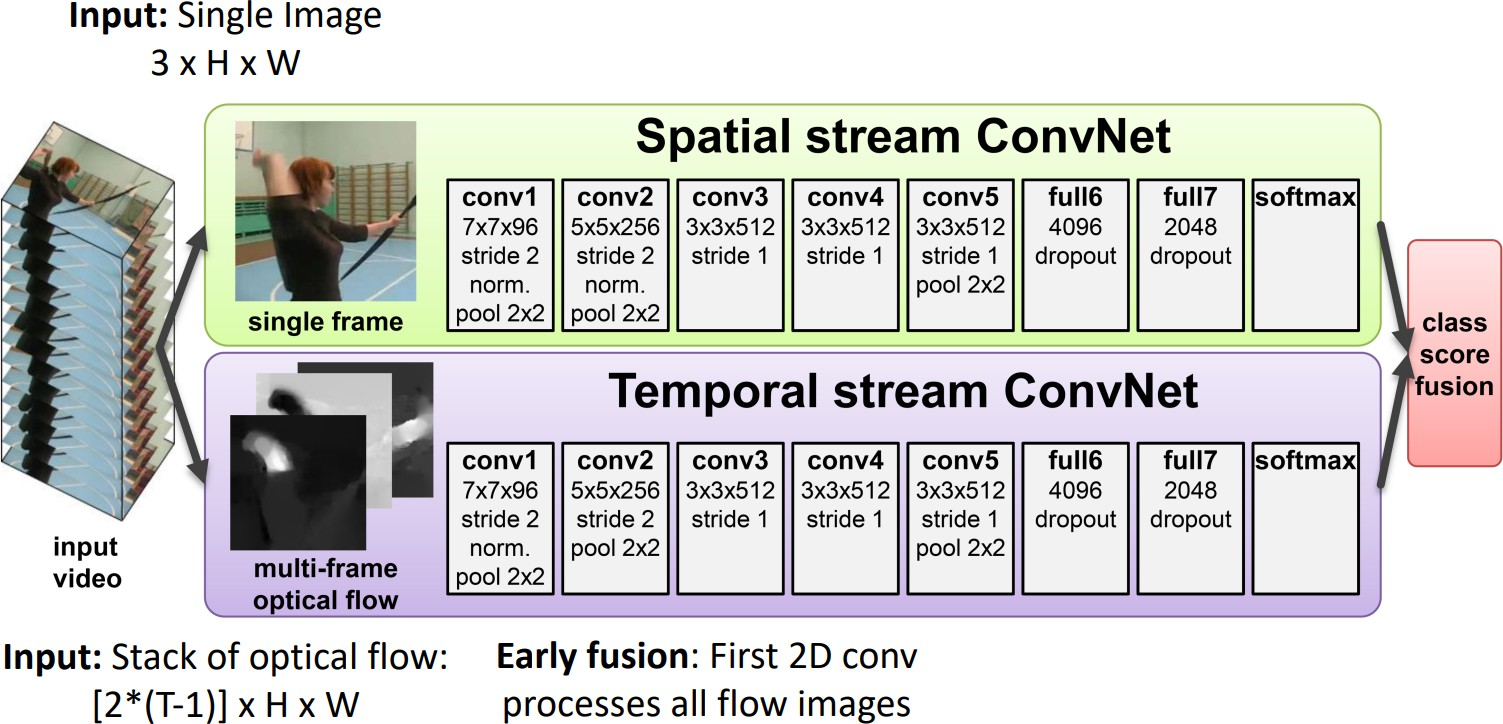
\includegraphics[width=1\textwidth,height=0.9\textheight,keepaspectratio]{images/video/slide_23_1_img.jpg}
    \end{figure}
\framebreak
    \begin{itemize}
        \item \textbf{RGB Stream:} Standard CNN (e.g., ResNet) for appearance features.
        \item \textbf{Optical Flow Stream:} Separate CNN for motion features.
        \item \textbf{Fusion:} Can be done at different stages:
        \begin{itemize}
            \item Early: Concatenate features from both streams.
            \item Late: Combine predictions from both streams.
        \end{itemize}
    \end{itemize}
\framebreak
    \begin{figure}
        \centering
        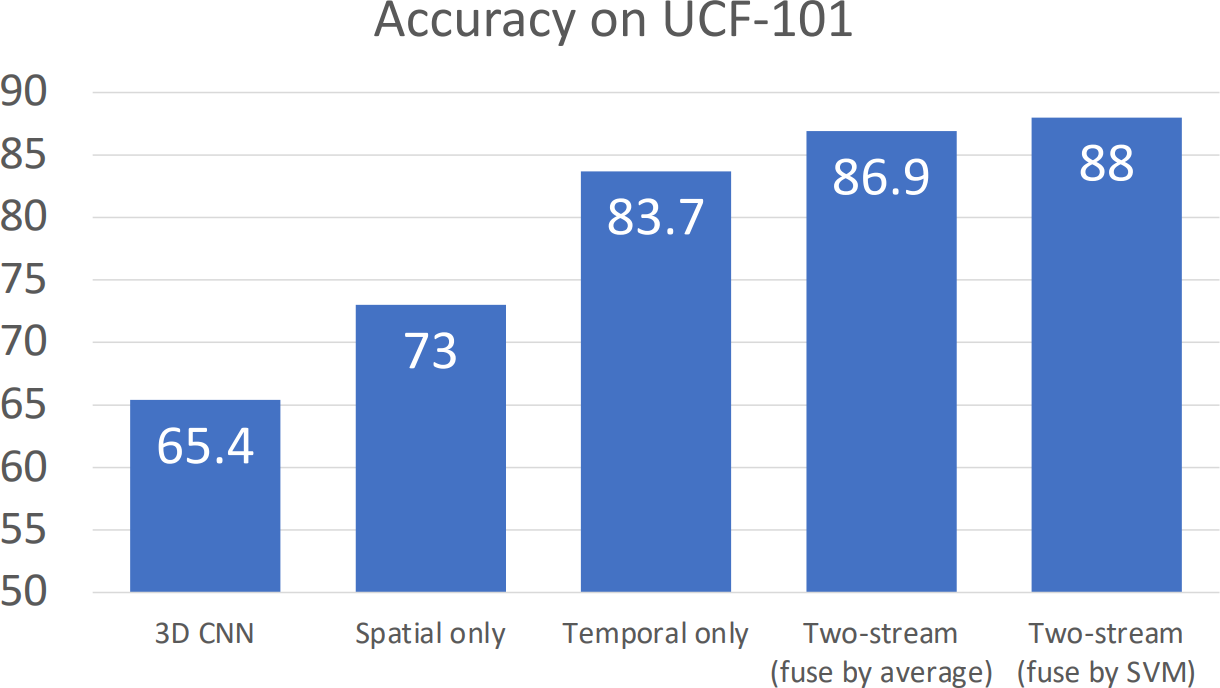
\includegraphics[width=1\textwidth,height=0.9\textheight,keepaspectratio]{images/video/slide_24_1_img.png}
    \end{figure}
\end{frame}
\subsection{Long-Term Temporal Structure}
\begin{frame}{Long-Term Temporal Structure}
    Understanding complex actions in videos often requires analyzing long-term temporal structure, rather than relying solely on short clips. This involves capturing dependencies and patterns that span extended periods, which are crucial for recognizing actions composed of multiple stages or events.

    \begin{itemize}
        \item \textbf{Temporal Segmentation:} Divides a video into meaningful segments based on changes in activity.
        \item \textbf{Temporal Action Proposals:} Identifies candidate time intervals where actions may occur.
    \end{itemize}

    These techniques enable models to focus on relevant portions of the video and improve the recognition of complex, long-duration actions.
\end{frame}

\begin{frame}{Modelling Long-Term Structure}
    Several approaches have been developed to effectively model long-term temporal dependencies in videos:

    \begin{itemize}
        \item \textbf{Hierarchical RNNs and LSTMs:} Stack multiple recurrent layers to capture both short-term and long-term dependencies at different temporal scales.
        \item \textbf{Temporal Segment Networks (TSN):} Sample frames or segments sparsely across the entire video and aggregate their representations to model long-range structure.
        \item \textbf{Memory Networks:} Utilize external memory modules to store and retrieve information across hundreds of frames, enabling reasoning over extended temporal contexts.
    \end{itemize}

    These methods help in recognizing actions that unfold over long durations and involve multiple stages.
\end{frame}

\begin{frame}{Modelling Long-Term Structure}
    \begin{itemize}
        \item So far, all our temporal CNNs only model local motion between frames in very short clips of approximately 2--5 seconds.
        \item What about long-term structure?
        \item<2-> \textbf{We know how to handle sequences!}
        \item<2-> How about \textbf{recurrent networks}?
    \end{itemize}
    \begin{figure}
        \centering
        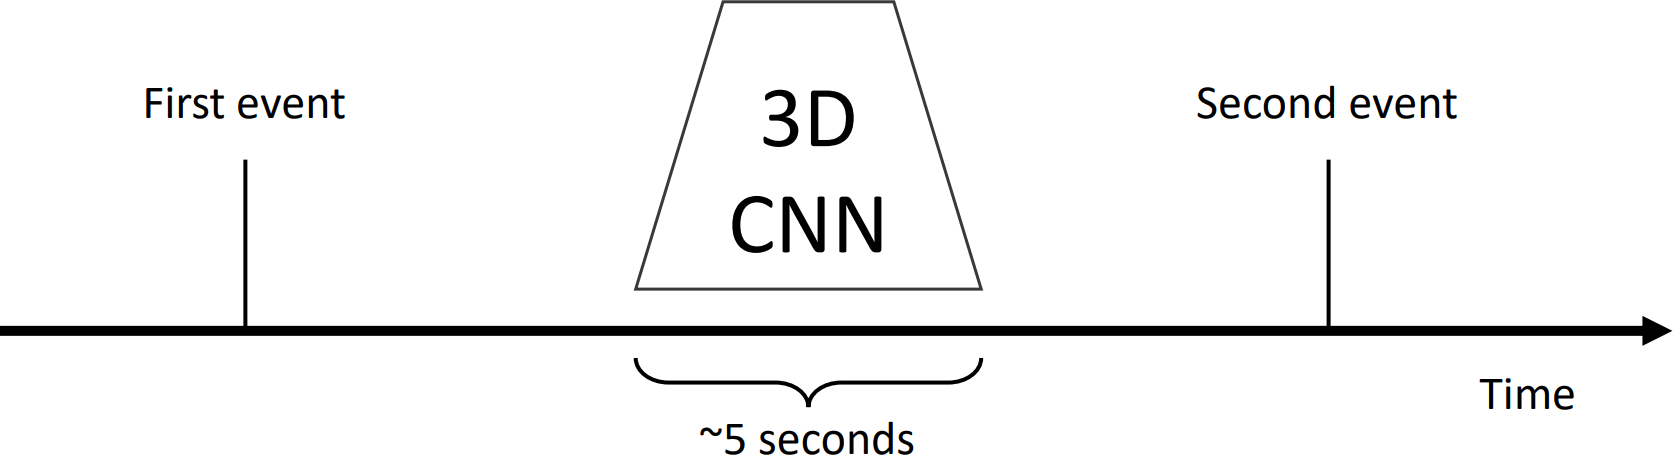
\includegraphics[width=1\textwidth,height=0.5\textheight,keepaspectratio]{images/video/slide_25_1_img.png}
    \end{figure}
\end{frame}

\begin{frame}{Modelling Long-Term Structure}
    \begin{itemize}
        \item Process local features using recurrent network (e.g. LSTM)
        \item Many to many: one output per video frame
    \end{itemize}
    \begin{figure}
        \centering
        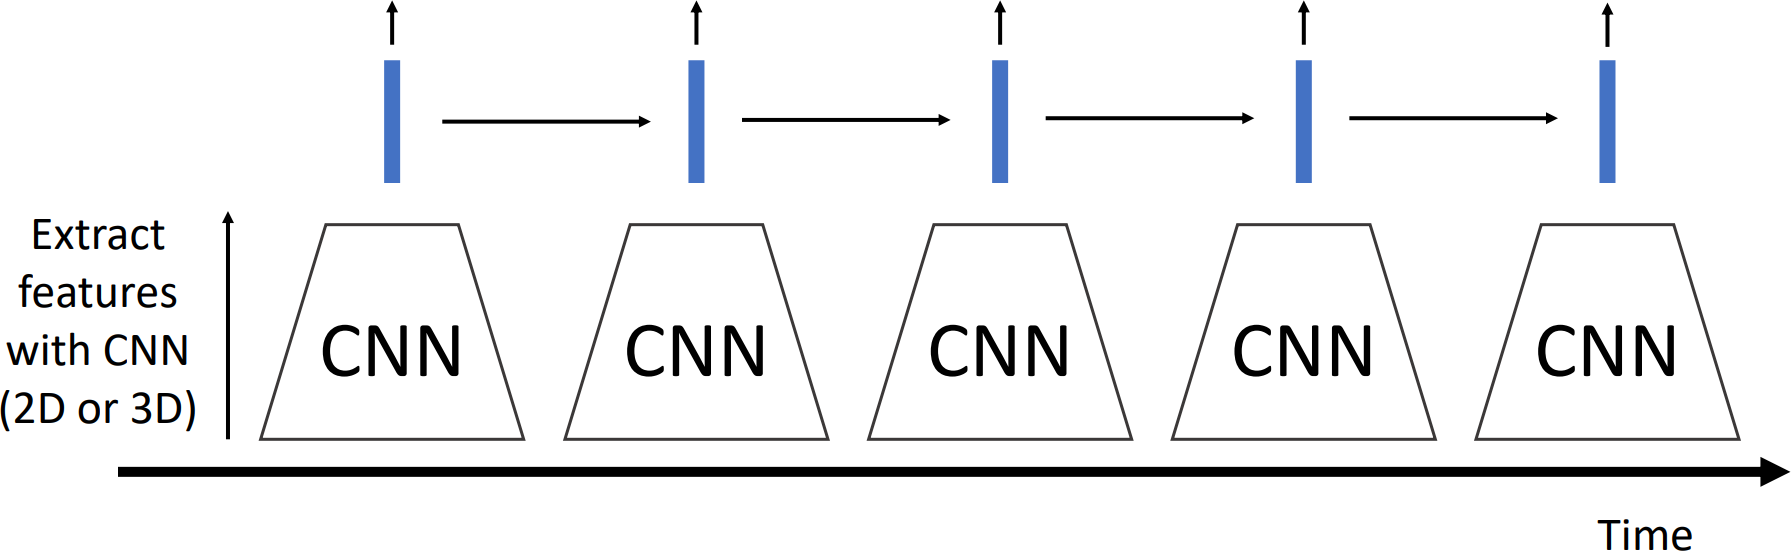
\includegraphics[width=1\textwidth,height=0.5\textheight,keepaspectratio]{images/video/slide_27_1_img.png}
    \end{figure}
\end{frame}

\begin{frame}[allowframebreaks]{Recurrent Convolutional Network}
    \begin{figure}
        \centering
        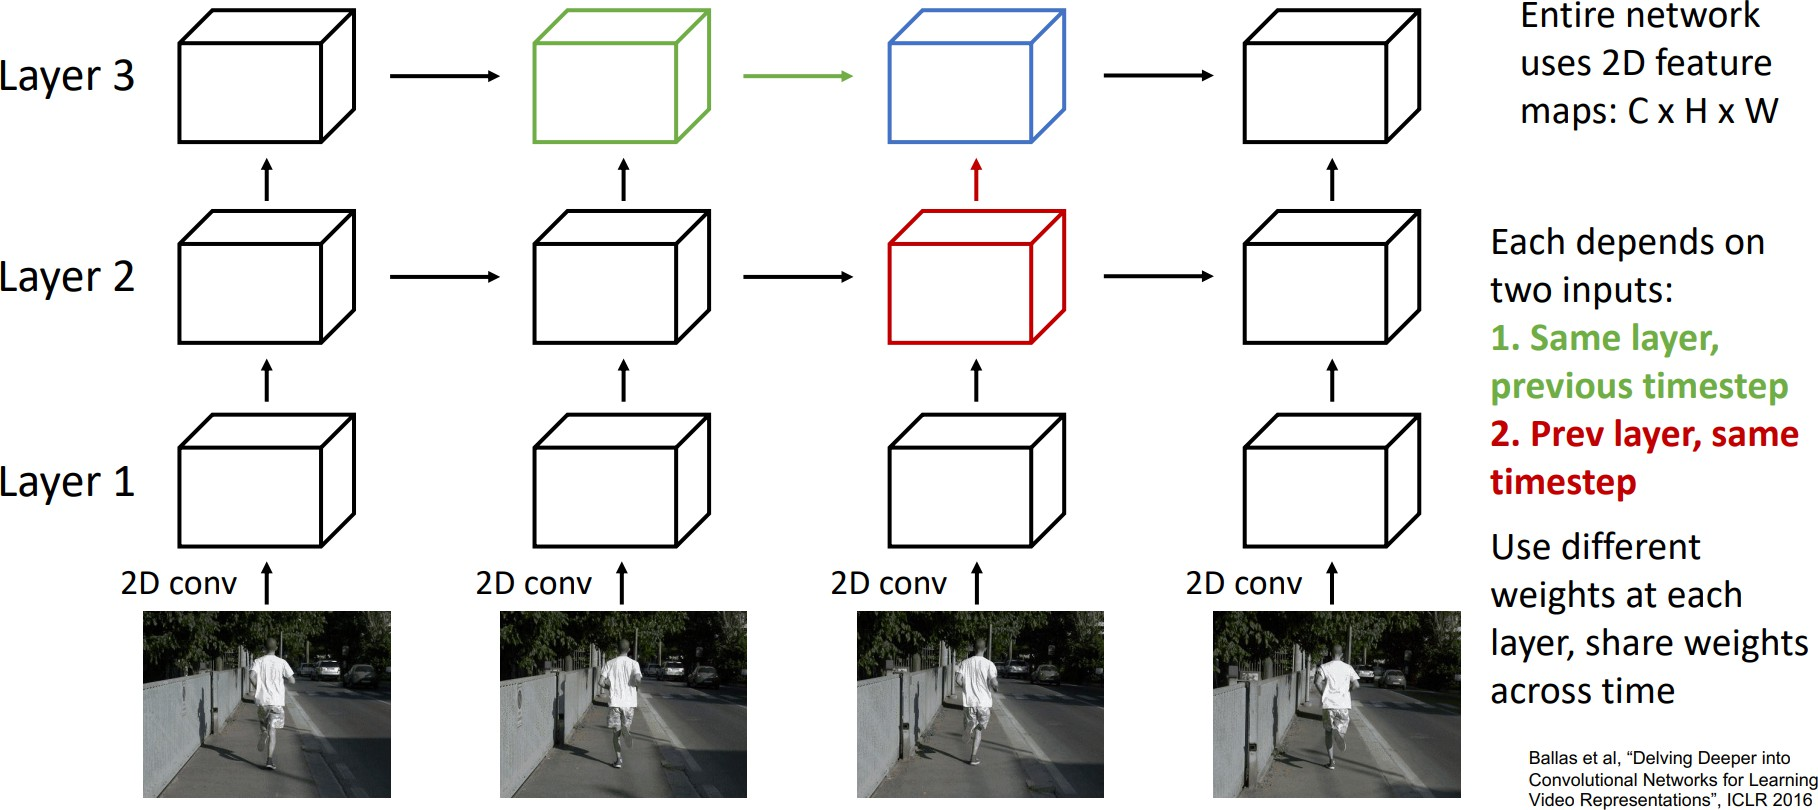
\includegraphics[width=1\textwidth,height=0.9\textheight,keepaspectratio]{images/video/slide_28_1_img.jpg}
    \end{figure}
\framebreak
    \begin{figure}
        \centering
        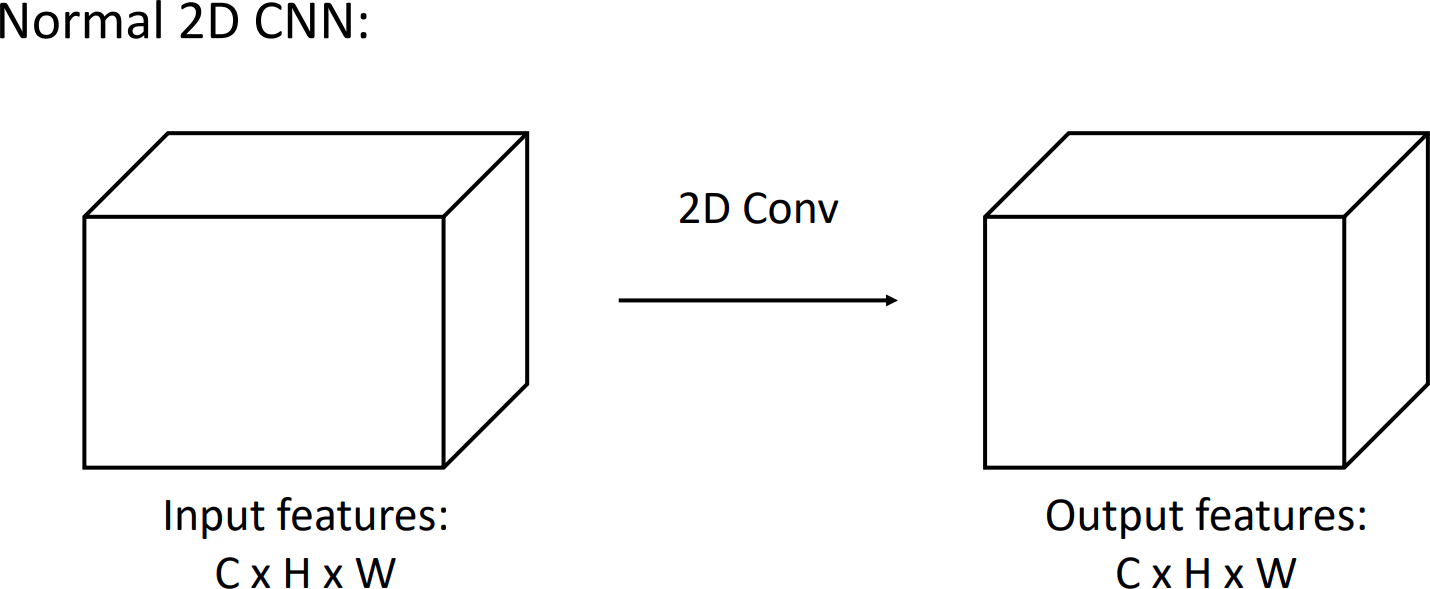
\includegraphics[width=1\textwidth,height=0.9\textheight,keepaspectratio]{images/video/slide_29_1_img.png}
    \end{figure}
\framebreak
    \begin{figure}
        \centering
        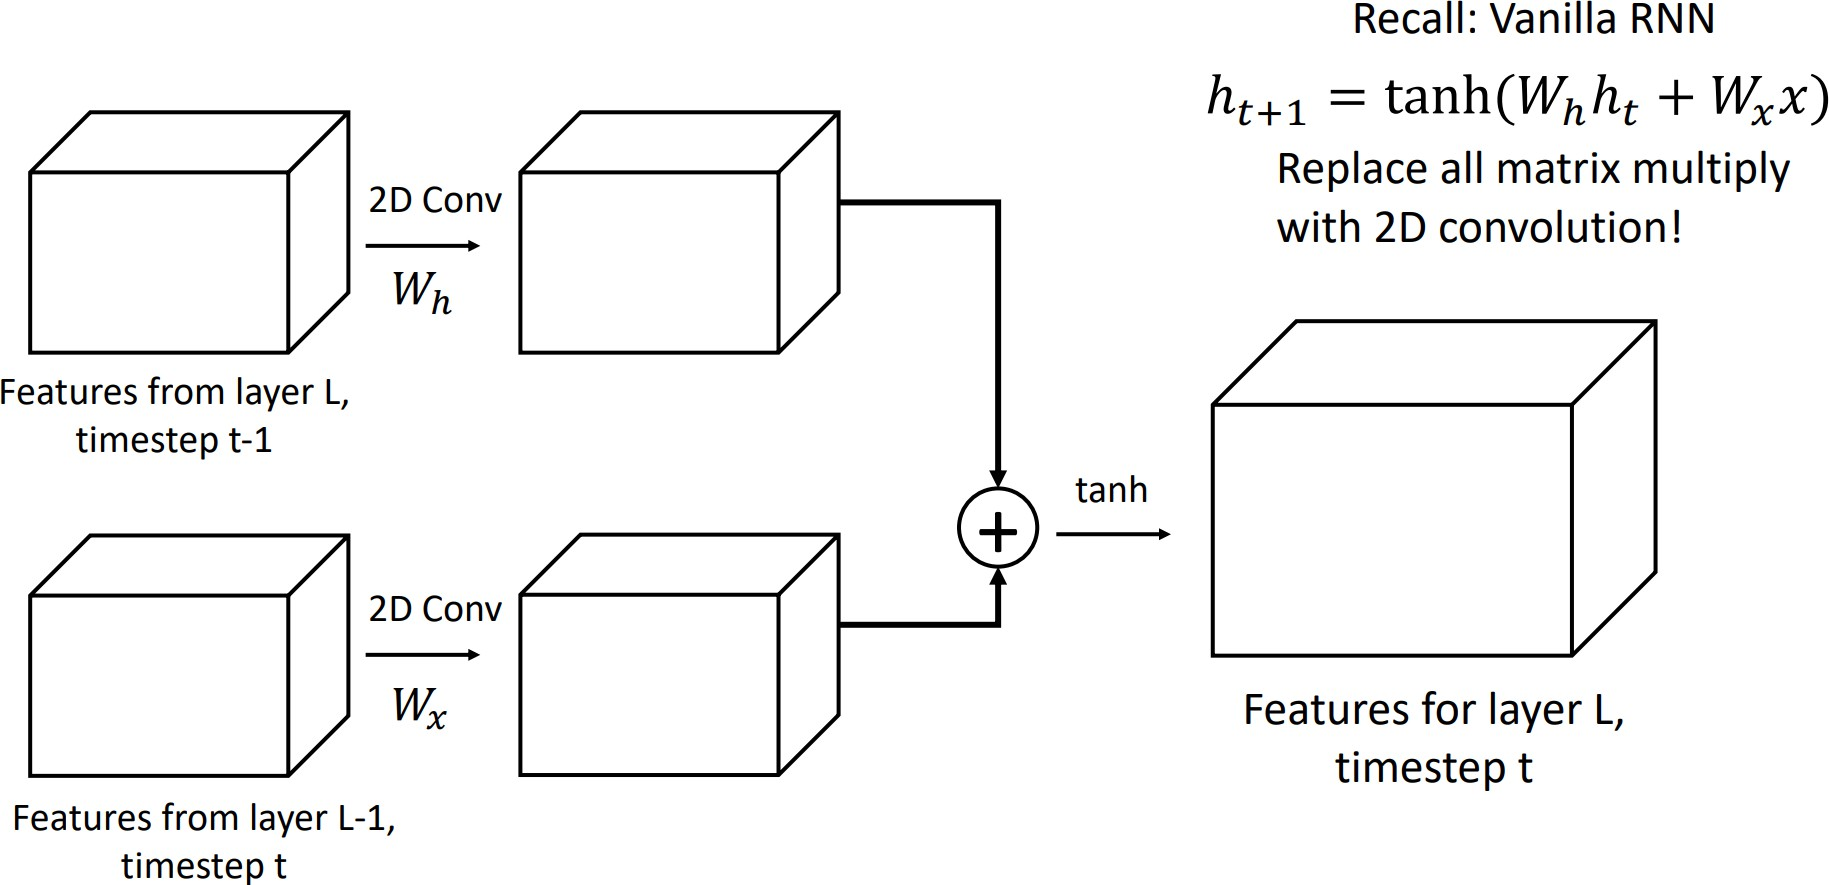
\includegraphics[width=1\textwidth,height=0.9\textheight,keepaspectratio]{images/video/slide_30_1_img.jpg}
    \end{figure}
\end{frame}

\begin{frame}[allowframebreaks]{Modeling long-term temporal structure}
    \begin{figure}
        \centering
        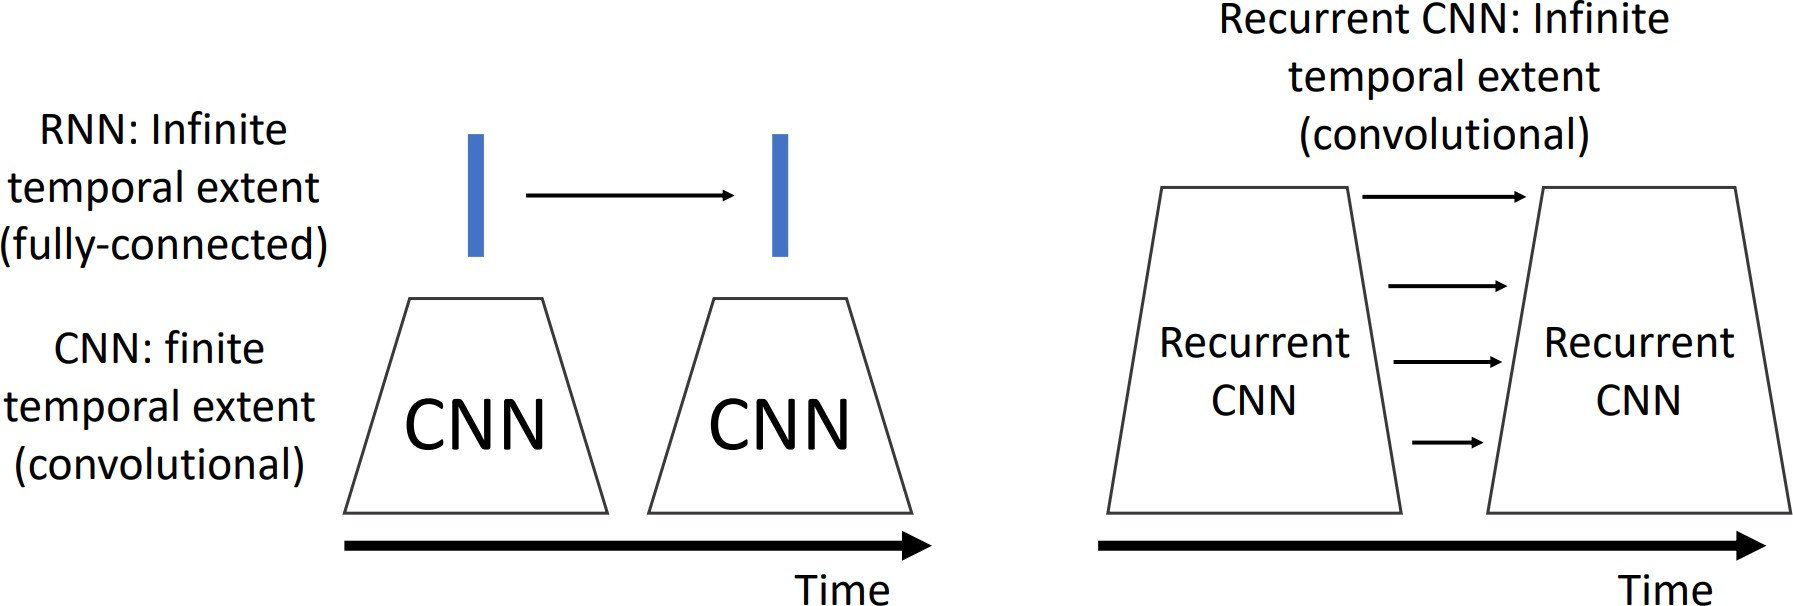
\includegraphics[width=1\textwidth,height=0.9\textheight,keepaspectratio]{images/video/slide_31_1_img.jpg}
    \end{figure}
\framebreak
    \begin{figure}
        \centering
        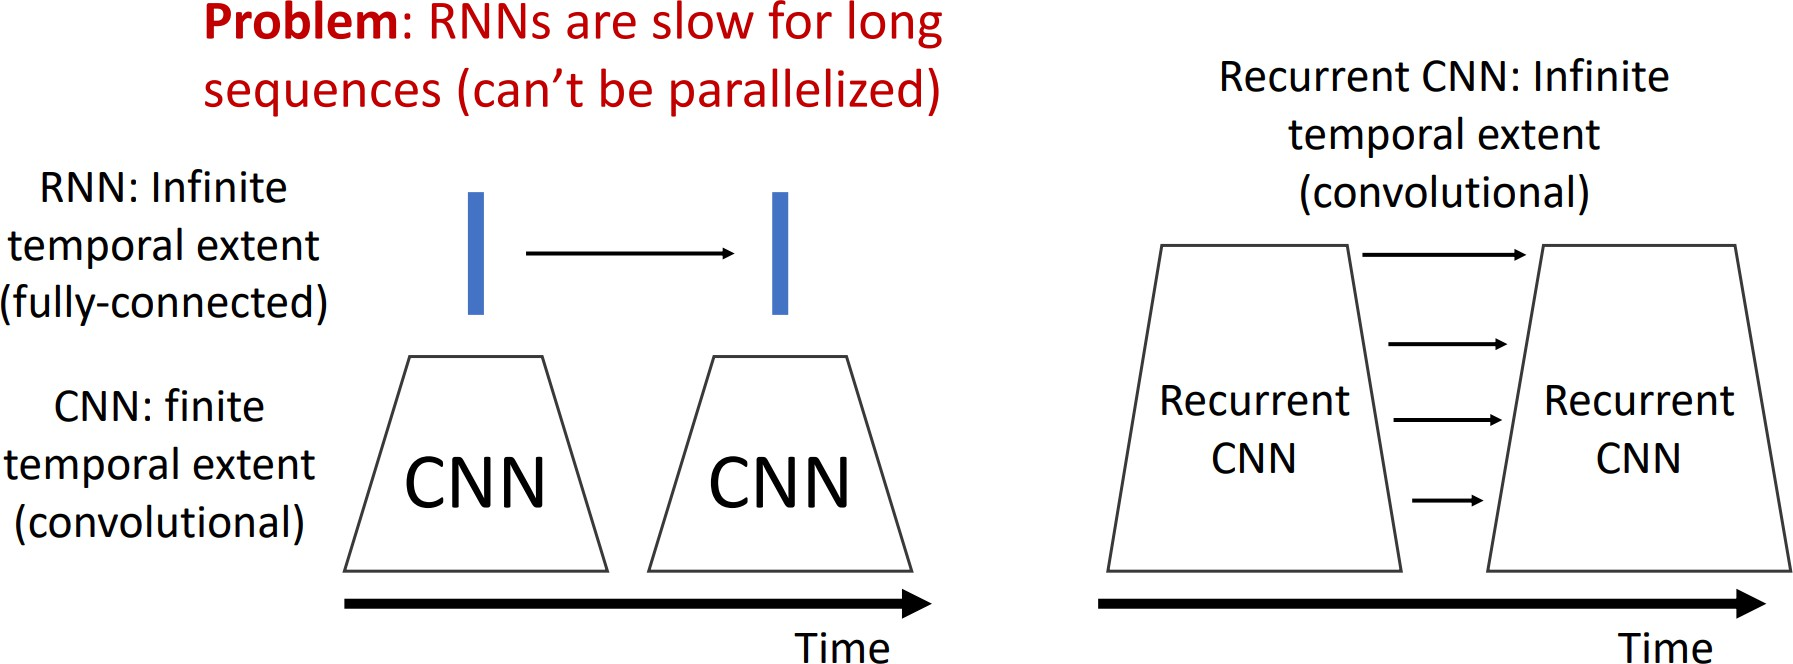
\includegraphics[width=1\textwidth,height=0.9\textheight,keepaspectratio]{images/video/slide_32_1_img.jpg}
    \end{figure}
\end{frame}
\subsection{Spatio-Temporal Self-Attention}
\begin{frame}[allowframebreaks]{Spatio-Temporal Self-Attention}
    \textbf{Spatio-Temporal Self-Attention} extends the Transformer architecture to video data by modeling dependencies across both spatial and temporal dimensions.

    \begin{itemize}
        \item \textbf{Transformers applied to video:} Video frames are treated as sequences, enabling the use of self-attention to capture relationships across space and time.
        \item \textbf{Factorized Attention (e.g., TimeSformer):} Attention is applied separately along spatial and temporal axes, reducing computational cost compared to full spatio-temporal attention.
        \item \textbf{Benefits:} Enables modeling of global context and long-range dependencies in videos.
        \item \textbf{Costs:} Self-attention has quadratic complexity with respect to sequence length, making it computationally expensive for long videos.
    \end{itemize}
\framebreak
    \begin{itemize}
        \item \textbf{Self-Attention Mechanism:} Captures long-range dependencies in both spatial and temporal dimensions.
        \item \textbf{Multi-Head Attention:} Allows the model to focus on different parts of the input sequence simultaneously.
    \end{itemize}
\end{frame}
\begin{frame}[allowframebreaks]{Spatio-Temporal Self-Attention (Nonlocal Block)}
    \begin{figure}
        \centering
        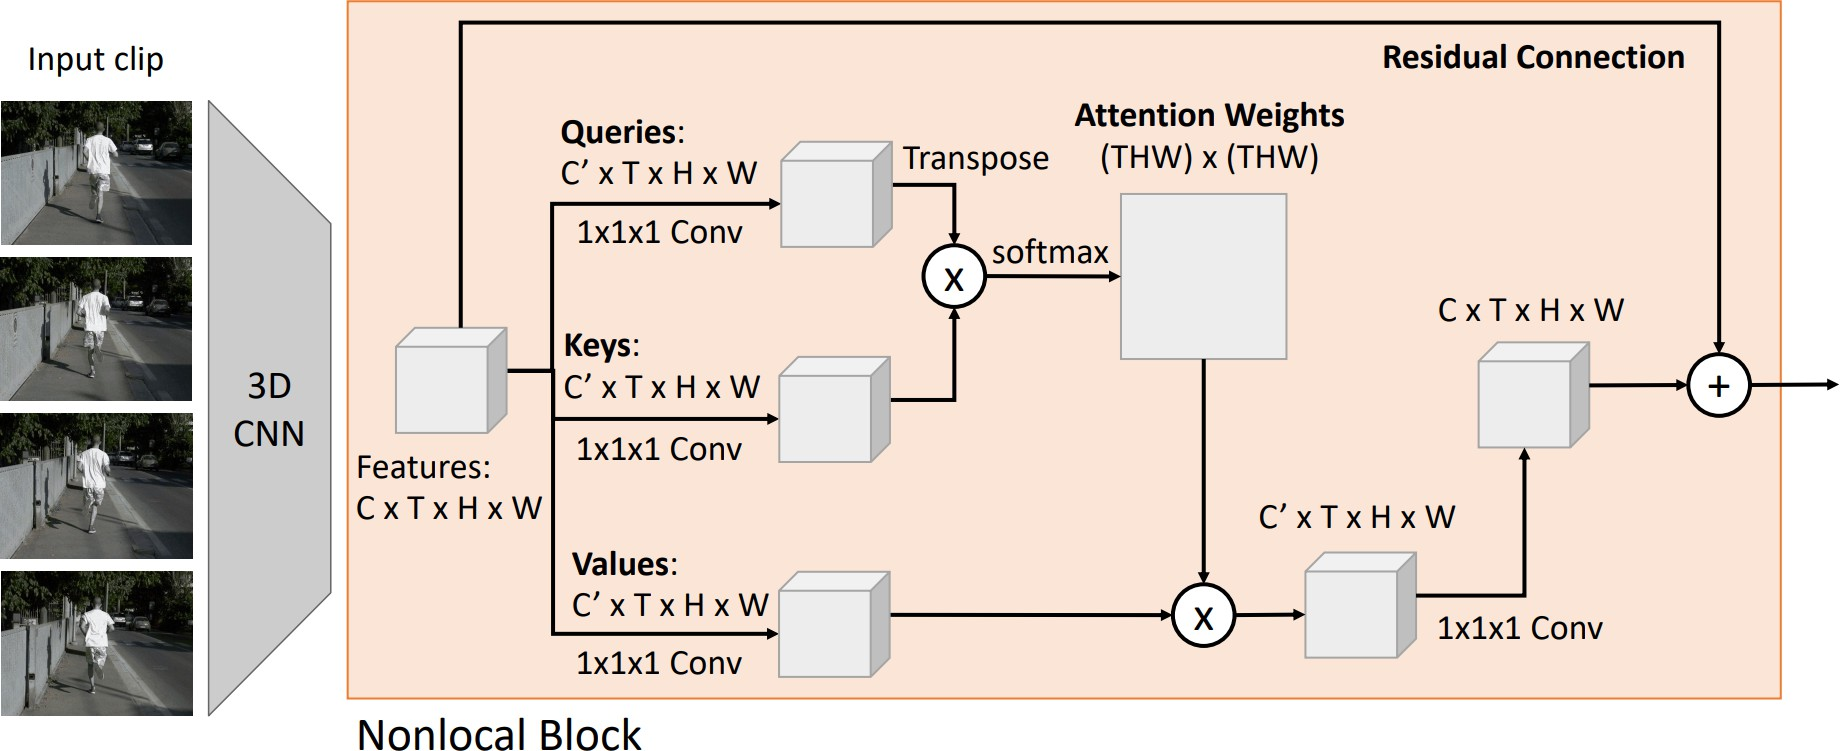
\includegraphics[width=1\textwidth,height=0.9\textheight,keepaspectratio]{images/video/slide_33_1_img.jpg}
    \end{figure}
\framebreak
    \begin{figure}
        \centering
        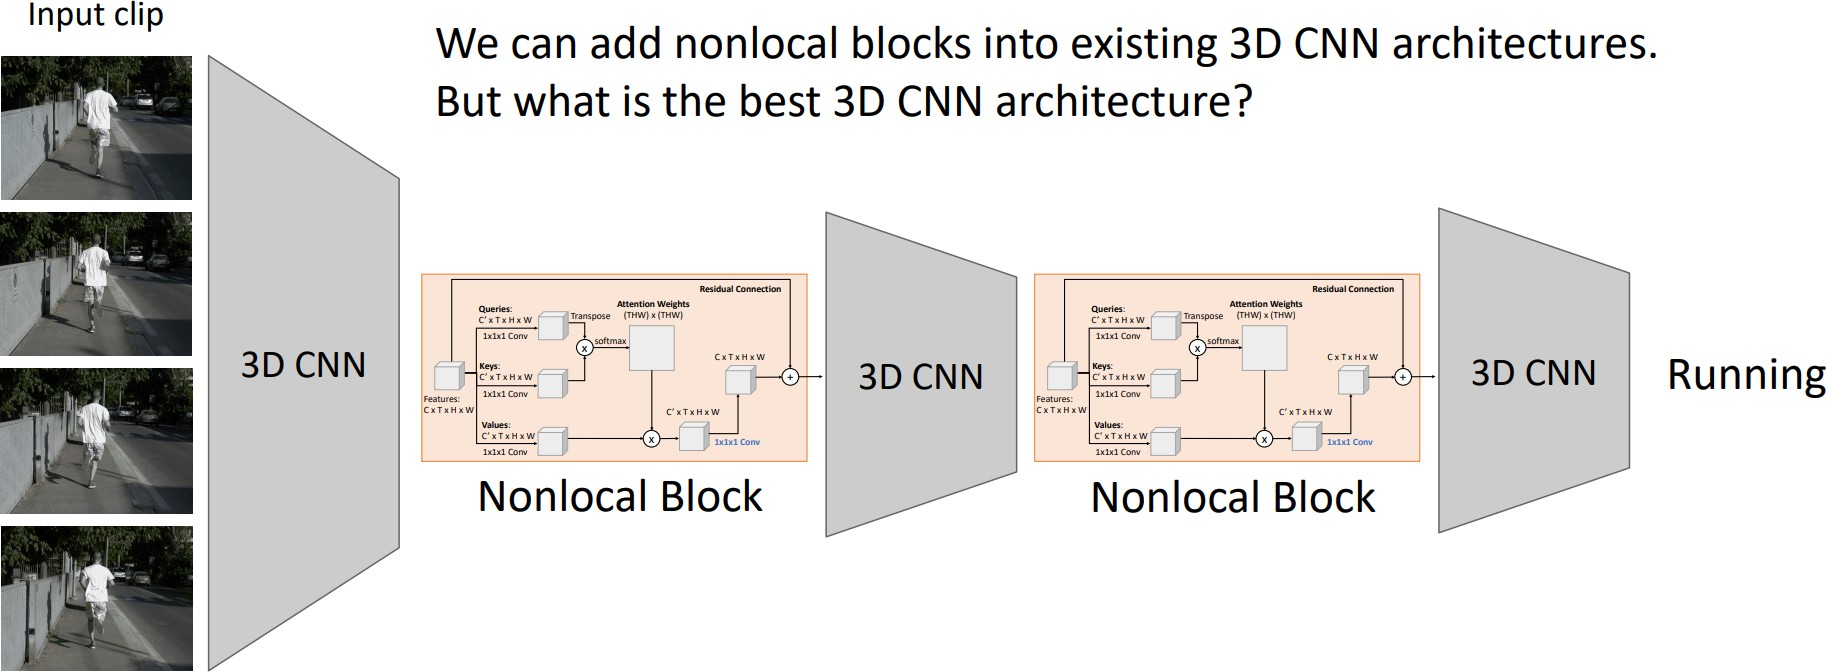
\includegraphics[width=1\textwidth,height=0.9\textheight,keepaspectratio]{images/video/slide_34_1_img.jpg}
    \end{figure}
\end{frame}
\subsection{I3D (Inflated 3D ConvNets)}
\begin{frame}[allowframebreaks]{Inflating 2D Networks to 3D (I3D)}
    \begin{itemize}
        \item There has been a lot of work on architectures for images.
        \item Can we reuse image architectures for video?
        \item Idea: take a 2D CNN architecture.
        \item Replace each 2D $K_h \times K_w$ conv/pool layer with a 3D $K_t \times K_h \times K_w$ version.
        \item Can use weights of 2D conv to initialize 3D conv: copy $K_t$ times in space and divide by $K_t$.
        \item This gives the same result as 2D conv given ``constant'' video input.
    \end{itemize}
\framebreak
    \begin{itemize}
        \item \textbf{Introduced by Carreira and Zisserman, CVPR 2017} \\
        \item \textbf{Key Ideas:}
        \begin{itemize}
            \item \textbf{Inflation of 2D Filters}: Converts 2D convolutional filters into 3D by replicating them across time.
            \item \textbf{Temporal Modeling}: Captures motion information effectively by leveraging pre-trained 2D networks.
            \item \textbf{End-to-End Training}: Trained on large video datasets, allowing transfer learning to new tasks.
            \item \textbf{Performance Boost}: Significantly improves action recognition accuracy compared to previous methods.
        \end{itemize}
    \end{itemize}
\framebreak
    \begin{figure}
        \centering
        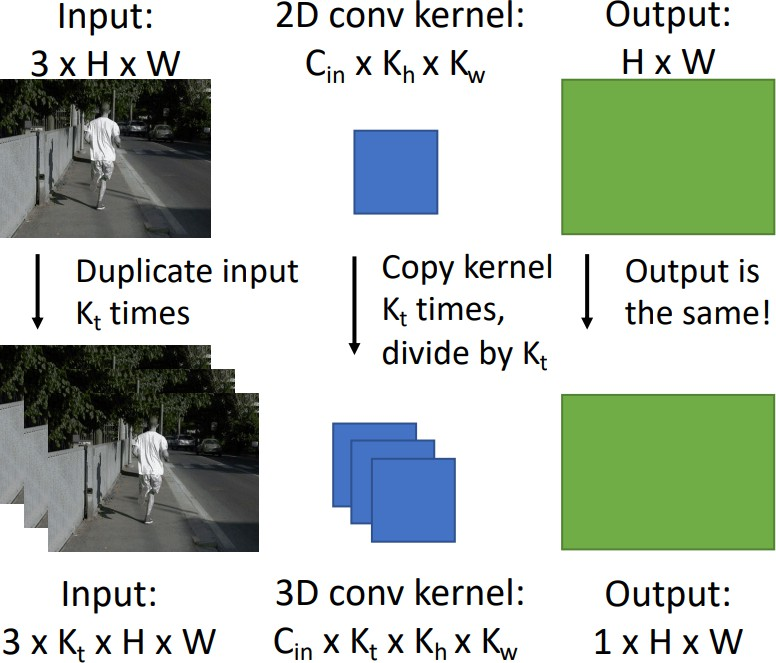
\includegraphics[width=1\textwidth,height=0.9\textheight,keepaspectratio]{images/video/slide_36_1_img.jpg}
    \end{figure}
\framebreak
    \begin{figure}
        \centering
        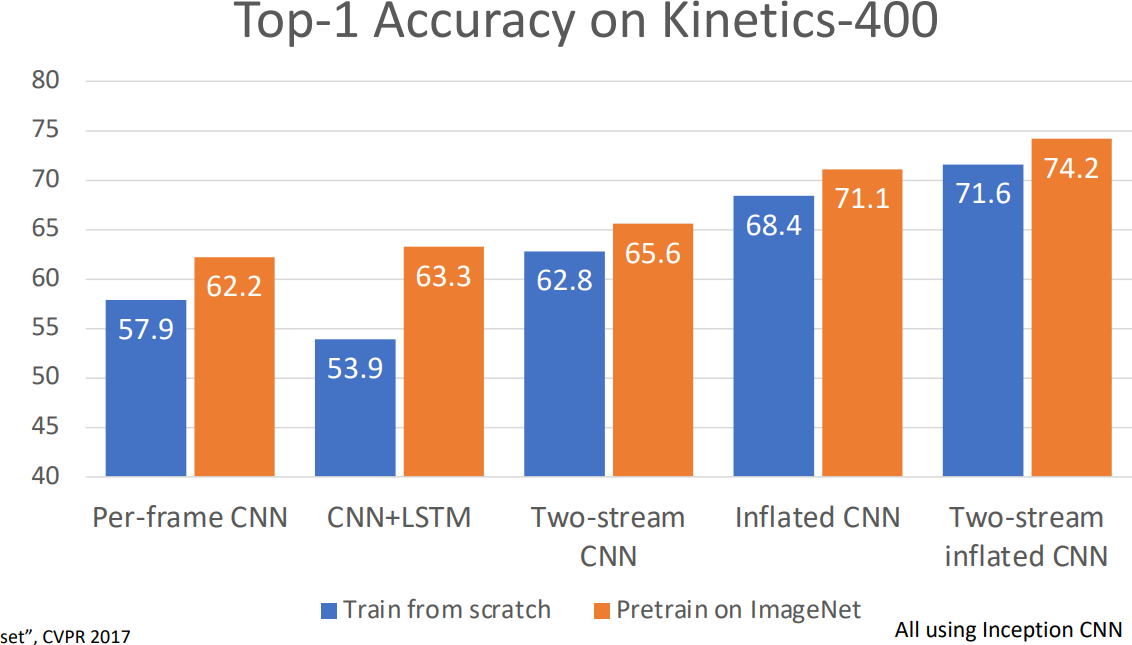
\includegraphics[width=1\textwidth,height=0.9\textheight,keepaspectratio]{images/video/slide_37_1_img.png}
    \end{figure}
\end{frame}
\subsection{Vision Transformers for Video}
\begin{frame}[allowframebreaks]{Vision Transformers for Video}
    \textbf{Vision Transformers (ViTs)} adapt the Transformer architecture for video data by treating video frames as sequences of patches, enabling the capture of long-range dependencies across both spatial and temporal dimensions.

    \begin{itemize}
        \item \textbf{Patch Embedding:} Each video frame is divided into patches, which are then linearly embedded into a sequence.
        \item \textbf{Temporal Encoding:} Positional encodings are added to capture temporal information.
        \item \textbf{Self-Attention Mechanism:} Allows the model to focus on different parts of the video sequence simultaneously.
        \item \textbf{Benefits:} Captures global context and long-range dependencies effectively.
        \item \textbf{Costs:} Computationally expensive due to quadratic complexity with respect to sequence length.
    \end{itemize}
\framebreak
    \begin{figure}
        \centering
        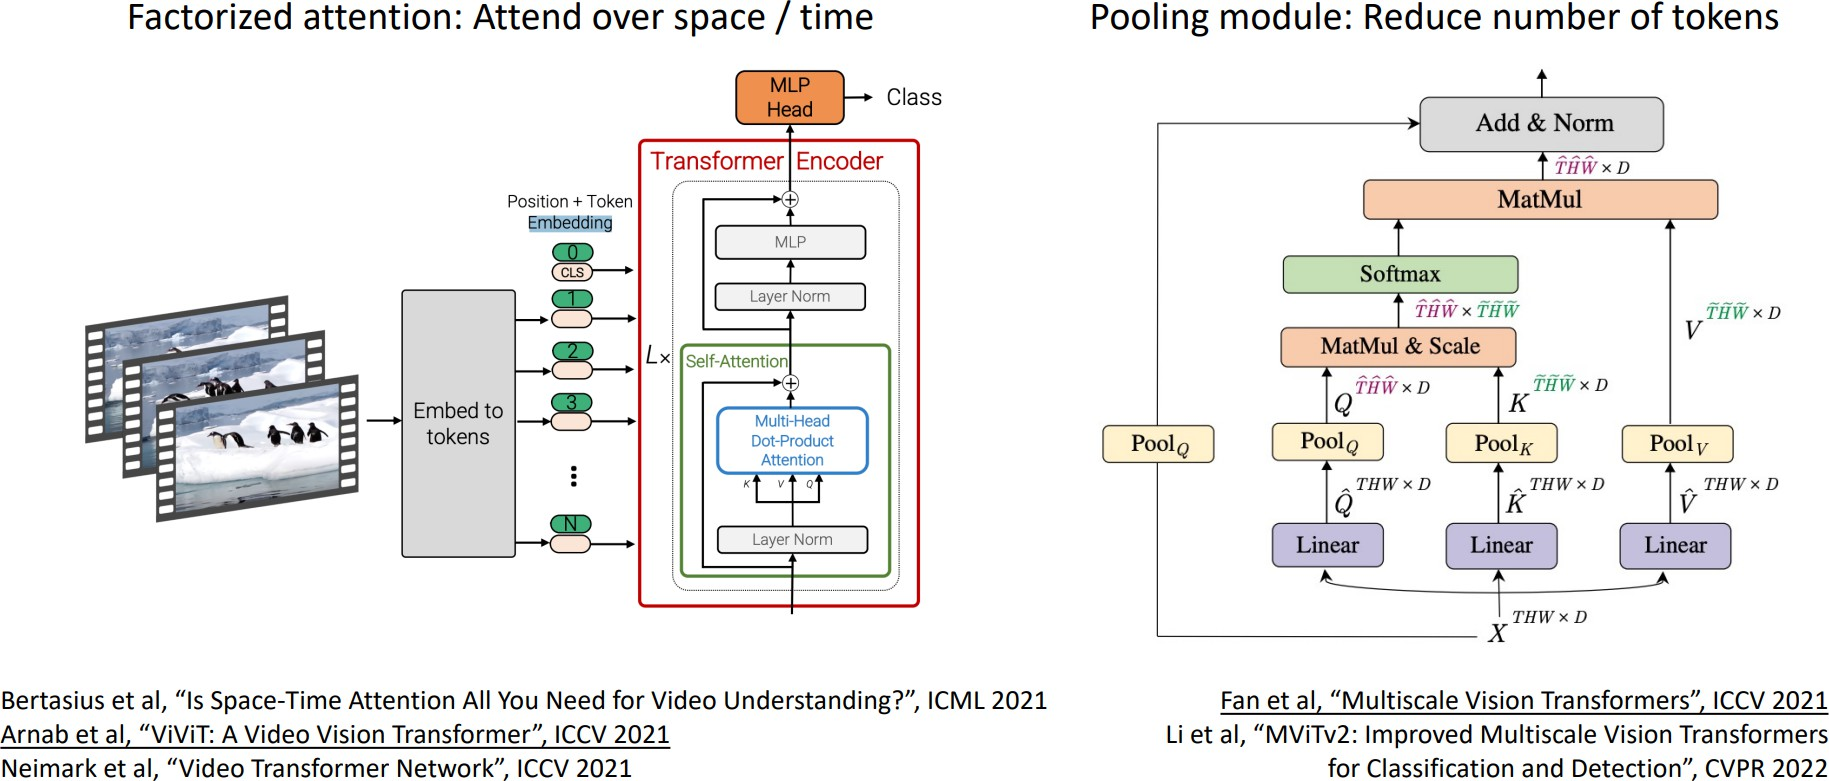
\includegraphics[width=1\textwidth,height=0.9\textheight,keepaspectratio]{images/video/slide_38_1_img.jpg}
    \end{figure}
\framebreak
    \begin{figure}
        \centering
        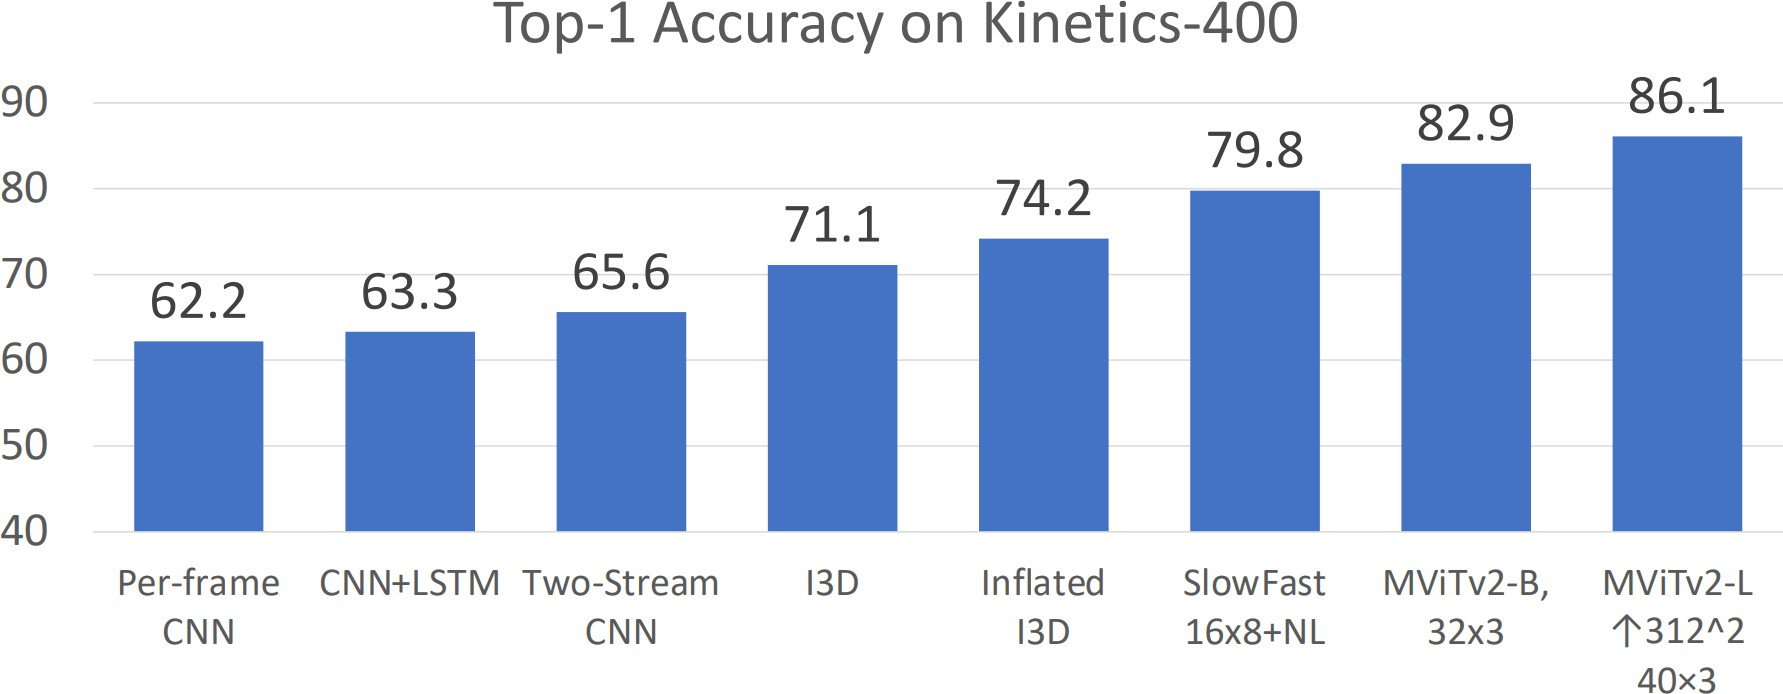
\includegraphics[width=1\textwidth,height=0.9\textheight,keepaspectratio]{images/video/slide_39_1_img.jpg}
    \end{figure}
\end{frame}

